%
% msa.tex -- visual representation of MSA
%
% (c) 2019 Prof Dr Andreas Müller, Hochschule Rapperswil
%
\documentclass[tikz]{standalone}
\usepackage{amsmath}
\usepackage{times}
\usepackage{txfonts}
\usepackage{pgfplots}
\usepackage{csvsimple}
\usetikzlibrary{arrows,intersections,math,fadings,shadings}
\begin{document}
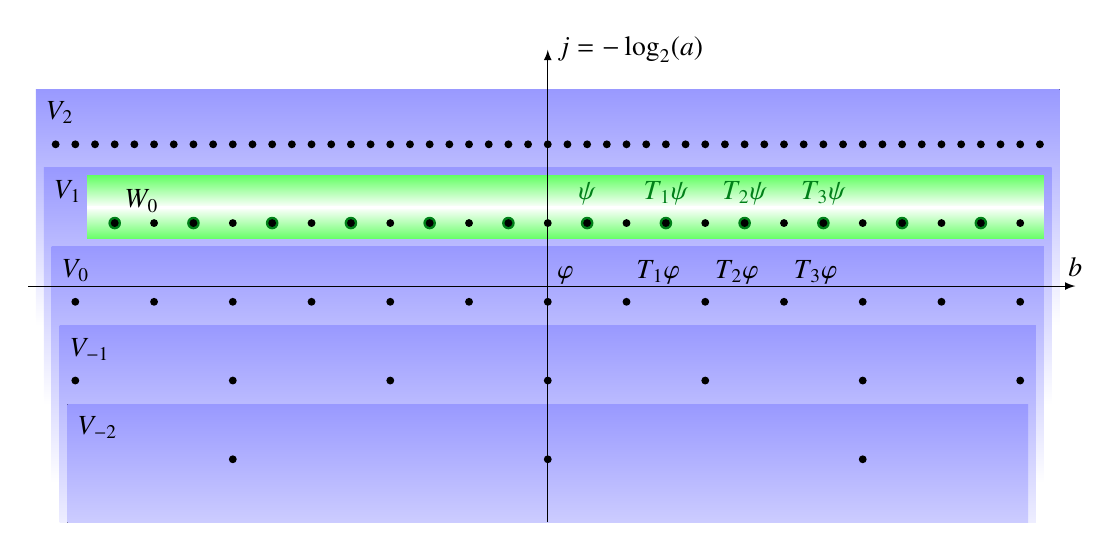
\begin{tikzpicture}[>=latex]

\definecolor{darkgreen}{rgb}{0,0.5,0.1}

\def\punkt#1#2{
	\fill #1 circle[radius=0.05];
}
\def\grau#1#2{
	\fill[color=gray!20] #1 circle[radius=0.05];
}

\def\zeile#1#2#3#4{
	\foreach \x in {{#1},...,{#2}}{
		%\punkt{({(\x+0.5)*#3},{#4-0.2})}{#3}
		\punkt{({(\x)*#3},{#4-0.2})}{#3}
	}
}
\def\zeilegrau#1#2#3#4{
	\foreach \x in {{#1},...,{#2}}{
		%\grau{({(\x+0.5)*#3},{#4-0.2})}{#3}
		\grau{({(\x)*#3},{#4-0.2})}{#3}
	}
}

\begin{scope}
\clip (-6.6,-3) rectangle (6.6,3);
\foreach \j in {2,...,-2}{
	\fill[top color=blue!40,bottom color=white]
		({-6.3-0.1*(\j)},{\j-2.5}) rectangle ({6.3+0.1*(\j)},{\j+0.5});
}
\end{scope}

\fill[top color=green!60,bottom color=white]
	(-5.85,1.0) rectangle (6.3,1.4);
\fill[bottom color=green!60,top color=white]
	(-5.85,0.6) rectangle (6.3,1.0);
\draw[color=white,line width=1pt] (-5.85,1)--(6.3,1);

\foreach \x in {-5.5,-4.5,...,5.5}{
	\fill[color=darkgreen] ({\x},0.8) circle[radius=0.08];
}

\zeile{-25}{25}{0.25}{2}
%\zeilegrau{-26}{-23}{0.25}{2}
\zeile{-11}{12}{0.5}{1}
%\zeilegrau{-13}{-11}{0.5}{1}
\zeile{-6}{6}{1}{0}
%\zeile{-6}{-6}{1}{0}
\zeile{-3}{3}{2}{-1}
\zeile{-1}{1}{4}{-2}
%\zeilegrau{-2}{-2}{4}{-2}

\draw[->,line width=0.3pt] (-6.6,0)--(6.7,0) coordinate[label=$b$];
\draw[->,line width=0.3pt] (0,-3)--(0,3) coordinate[label={right:$j=-\log_2(a)$}];

\node at (0.0,-0.1) [above right] {$\varphi$};
\node at (1.0,-0.1) [above right] {$T_1\varphi$};
\node at (2.0,-0.1) [above right] {$T_2\varphi$};
\node at (3.0,-0.1) [above right] {$T_3\varphi$};

\node[color=darkgreen] at (0.5,0.9) [above] {$\psi$};
\node[color=darkgreen] at (1.5,0.9) [above] {$T_1\psi$};
\node[color=darkgreen] at (2.5,0.9) [above] {$T_2\psi$};
\node[color=darkgreen] at (3.5,0.9) [above] {$T_3\psi$};

\node at (-6.5,2.2) [right] {$V_2$};
\node at (-6.4,1.2) [right] {$V_1$};
\node at (-5.5,1.08) [right] {$W_0$};
\node at (-6.3,0.2) [right] {$V_0$};
\node at (-6.2,-0.8) [right] {$V_{-1}$};
\node at (-6.1,-1.8) [right] {$V_{-2}$};

\end{tikzpicture}
\end{document}

